\begin{figure}[!h]
  \centering

  \begin{subfigure}{\textwidth}
    \centering
    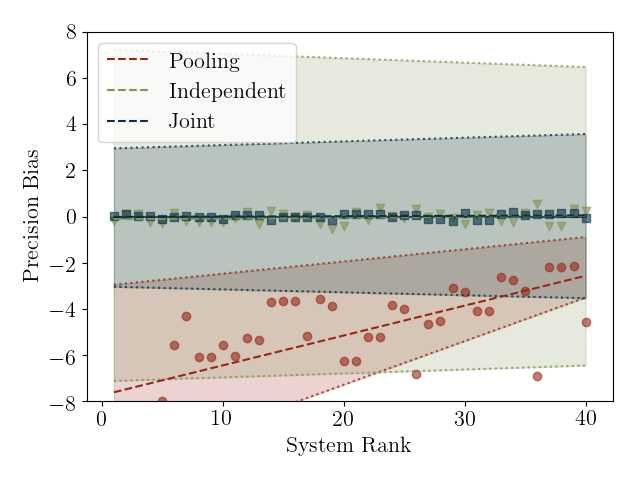
\includegraphics[width=0.8\textwidth]{figures/simulation/simulation-p}
    \caption{}
  \end{subfigure}

  \begin{subfigure}{\textwidth}
    \centering
    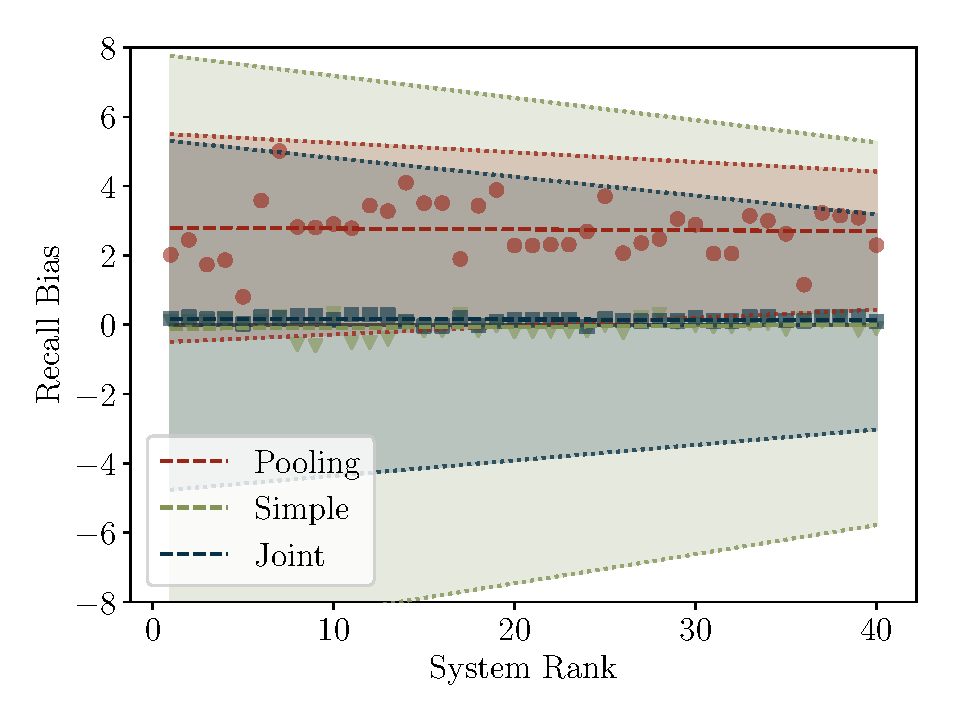
\includegraphics[width=0.8\textwidth]{figures/simulation/simulation-r}
    \caption{}
  \end{subfigure}

  \caption[Reduction of variance with the importance-reweighted estimator]{\label{fig:simulation}
  A comparison of bias for the pooling, simple and joint estimators on the TAC KBP 2015 challenge.
  Each point in the figure is a mean of 500 repeated trials; dotted lines show the 90\% quartile.
  %The pooling based method uses between 5,000 and 6,000 labeled instances, while the sampling based methods use 
  %approximately 150 samples from each system.
  %Dashed trend lines indicate the mean bias of the estimation method: 
  %Unbiased estimates lie on the $y = x$ line.
  Both the simple and joint estimators are unbiased, and the joint estimator is able to significantly reduce variance.
  }
\end{figure}


\begin{figure}[!h]
  \centering
  \begin{subfigure}{\textwidth}
    \centering
    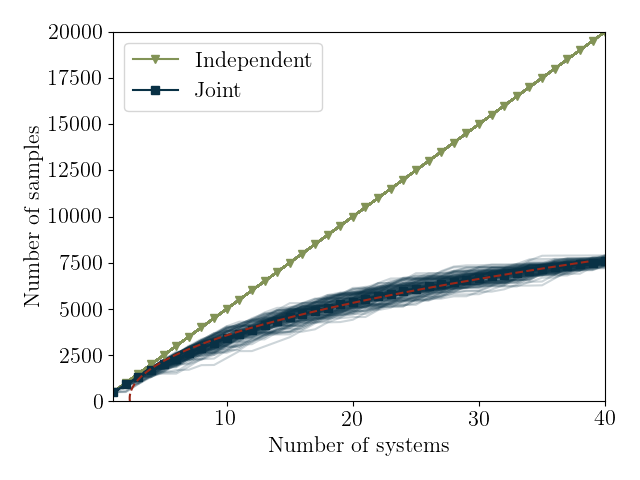
\includegraphics[width=0.8\textwidth]{figures/simulation/simulation-n}
    \caption{}
  \end{subfigure}

  \begin{subfigure}{0.49\textwidth}
    \centering
    \begin{figure*}[th]
  \centering
  \begin{subfigure}[b]{0.45\textwidth}
  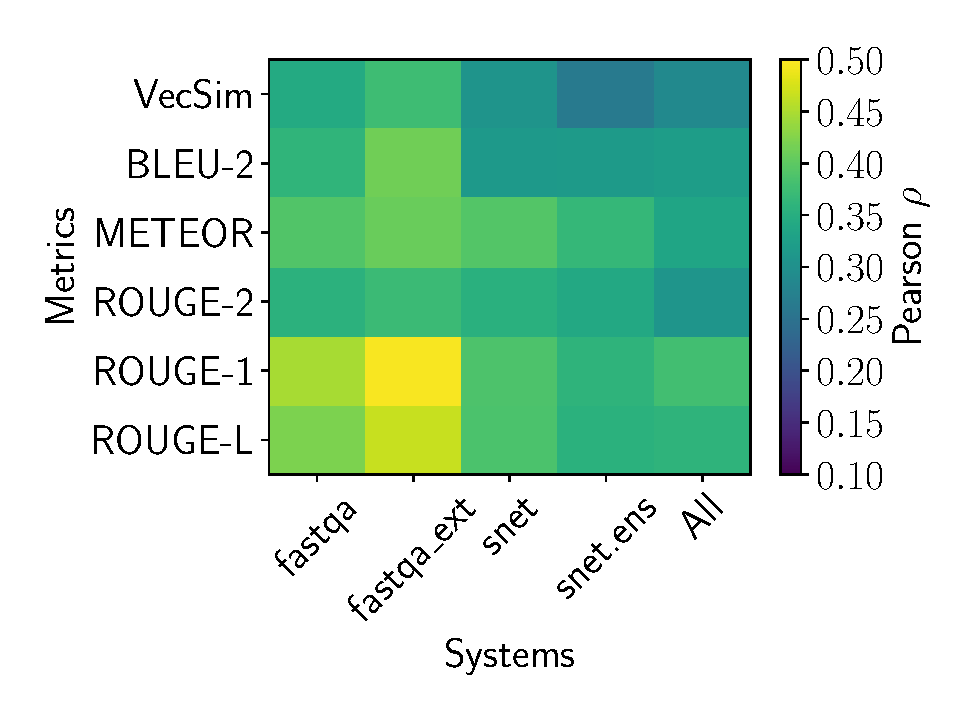
\includegraphics[width=\textwidth]{figures/msmarco_correlation}
  \caption{MS MARCO with the \texttt{AnyCorrect} prompt}
  \end{subfigure} \hfill
  \centering
  \begin{subfigure}[b]{0.45\textwidth}
  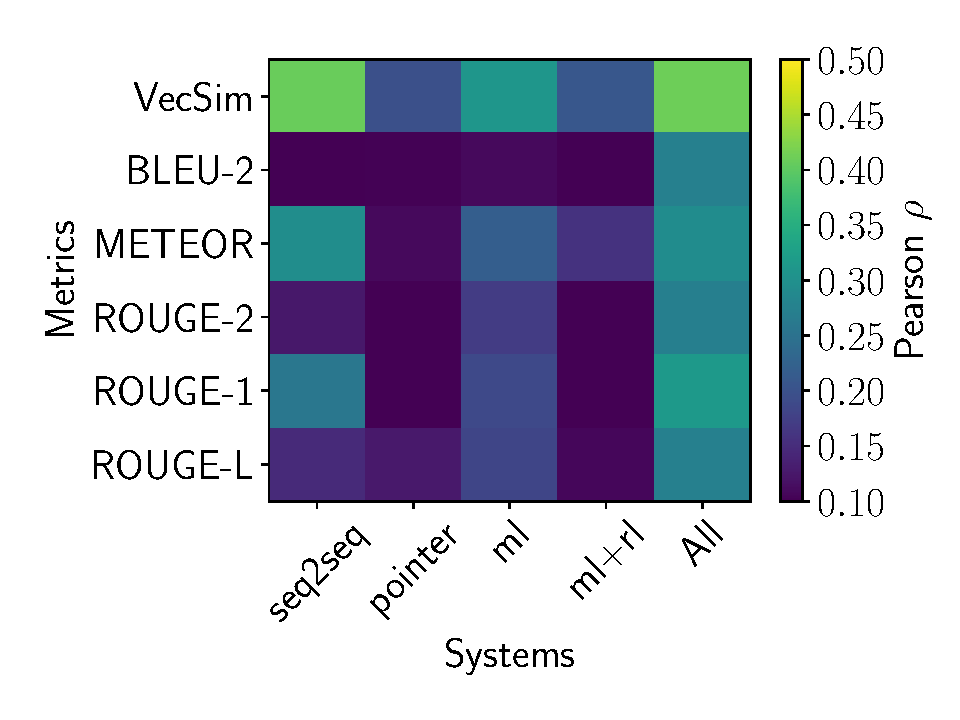
\includegraphics[width=\textwidth]{figures/lqual_correlation}
  \caption{CNN/Daily Mail with the \texttt{Edit} prompt}
  \end{subfigure}
  \caption{\label{fig:correlation} Correlations of different automatic metrics on the MS MARCO and CNN/Daily Mail tasks.
  Certain systems are more correlated with certain automatic metrics than others, but overall the correlation is low to moderate for most systems and metrics.
  }
\end{figure*}


\section{\label{sec:evaluation}Experimental results}

We are now ready to evaluate the performance of our control variates estimator proposed in \refsec{method} using the datasets presented in \refsec{tasks}.
Recall that our primary quantity of interest is \textit{data efficiency}, the ratio of the number of human judgments required to estimate the overall human evaluation score for the control variates estimator versus the sample mean.
We'll briefly review the automatic metrics used in our evaluation before analyzing the results.

%\begin{figure}[t]
%  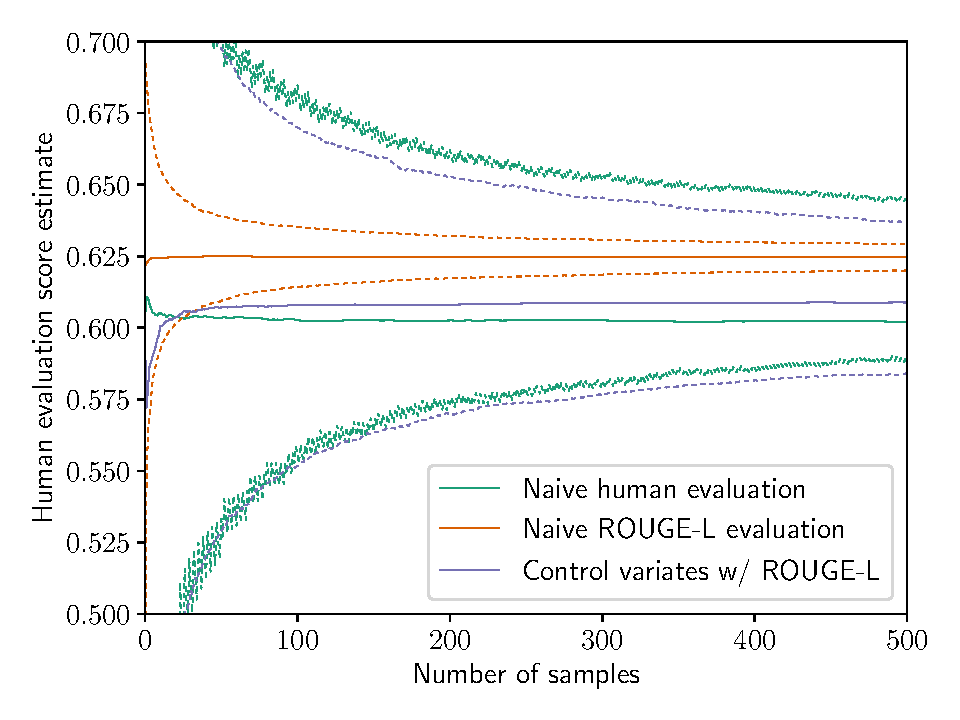
\includegraphics[width=\columnwidth]{figures/msmarco_full_trajectory}
%  \caption{\label{fig:bias-trajectory} A comparison of the human score estimates made by (a) naively sampling humans, (b) scaling and shifting the best automatic metric (ROUGE-L) and (c) incorporating the automatic metric into the control variates estimator proposed in this paper.
%  While (c) does not significantly reduce variance in its estimates, it is still an unbiased estimation of the human evaluation score, unlike (b).
%  The low confidence interval for the ROUGE-L scores are because they do not observe any annotator noise.
%  \ac{The curves are not exactly aligned because of a minor error in data for this plots. It will be fixed.}
%  }
%\end{figure}

% Evaluation
\paragraph{Automatic metrics.}
We consider the following frequently used automatic word-overlap based metrics in our work:
\textbf{BLEU}~\citep{papineni02bleu}, \textbf{ROUGE}~\citep{lin2004rouge} and \textbf{METEOR}~\citep{lavie2009meteor}.
Following \citet{novikova2017why} and \citet{liu2016evaluate}, we also compared a vector-based sentence-similarity using \texttt{sent2vec}~\citep{pagliardini2017unsupervised} to compare sentences (\textbf{VecSim}).
\reffig{correlation} shows how each of these metrics is correlated with human judgment for the systems being evaluated.
Unsurprisingly, the correlation varies considerably across systems, with token-based metrics correlating more strongly for systems that are more extractive in nature (\texttt{fastqa} and \texttt{fastqa\_ext}).

%\reffig{bias-trajectory} shows a trajectory estimates for human evaluation scores using the baseline of naive human evaluation versus those with the proposed control variates method.\footnote{%
%  All confidence intervals reported here are measured using 5,000 bootstrap samples generated by picking uniformly from the examples from the system output and then uniformly from the human annotations on that example.
%  }
%We also plot the estimate produced using an automatic metric, namely ROUGE-L after being scaled and shifted to match human evaluation scores at the system-level.
%Here, we see that while the control variates approach does not significantly reduce variance in estimates, it remains unbiased when using the model, unlike using the automatic metric.

%\begin{figure*}[t]
%  \centering
%  \begin{subfigure}[b]{0.45\textwidth}
%    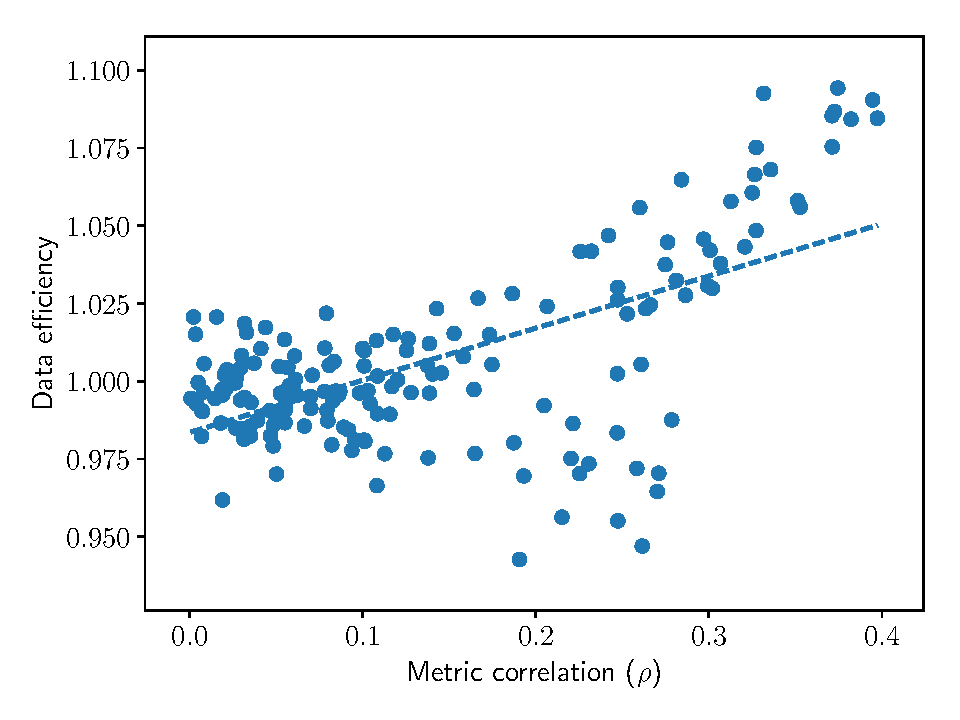
\includegraphics[width=\textwidth]{figures/de_vs_rho}
%  \end{subfigure} \hfill
%  \begin{subfigure}[b]{0.45\textwidth}
%    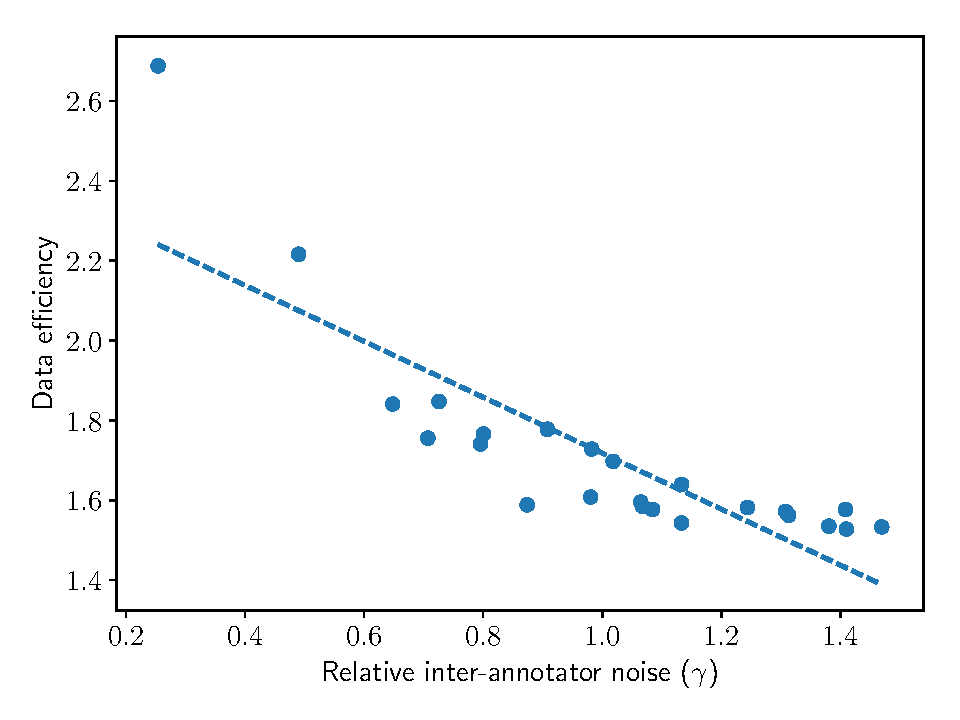
\includegraphics[width=\textwidth]{figures/de_vs_gamma}
%  \end{subfigure}
%  \caption{\label{fig:data-efficiency} A comparison of data efficiency possible across different systems and metrics. \ac{This figure seems like not very important so prefer ignoring.}}
%\end{figure*}

\begin{figure*}[th]
  \centering
  \begin{subfigure}[b]{0.32\textwidth}
  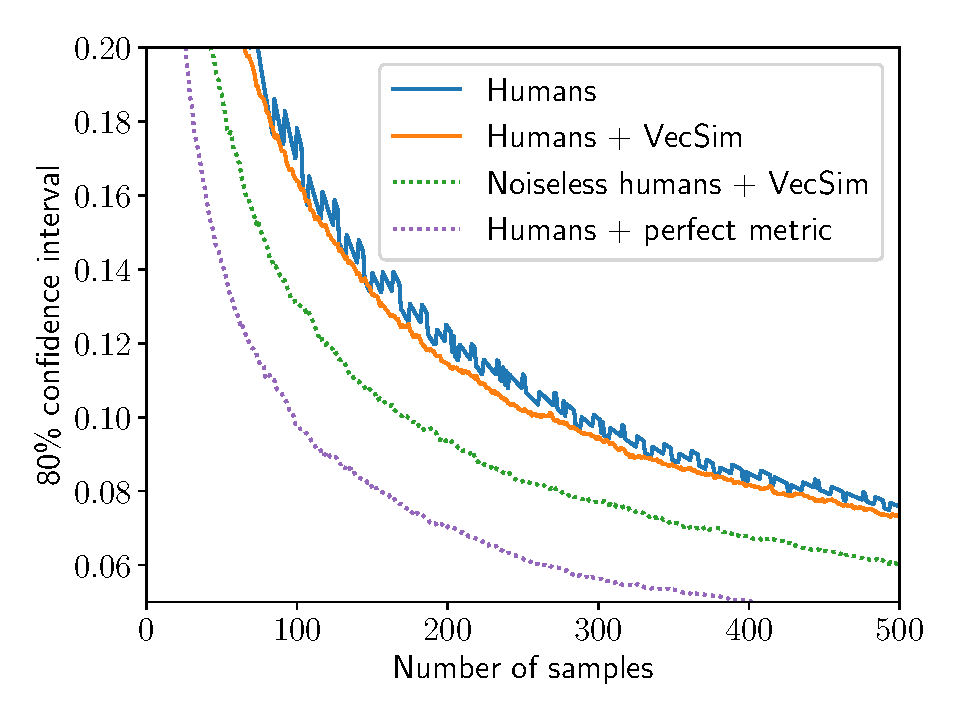
\includegraphics[width=\textwidth]{figures/lqual_trajectory_foil}
    \caption{\label{fig:trajectory-a}\texttt{seq2seq} on CNN/Daily Mail using the \texttt{Overall}}
  \end{subfigure} 
  \hfill
  \begin{subfigure}[b]{0.32\textwidth}
  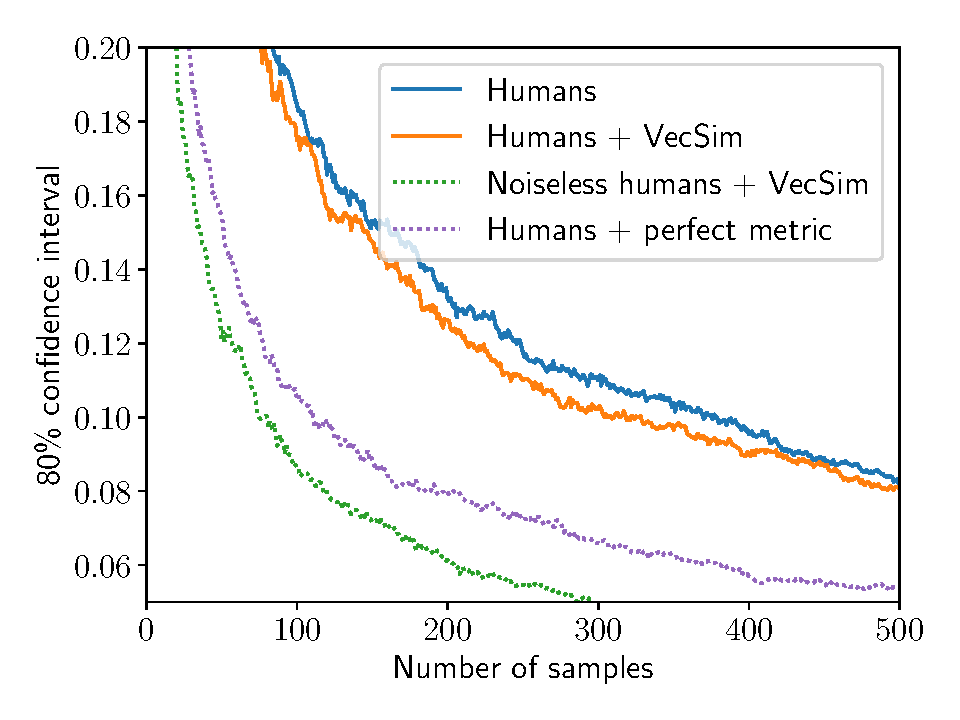
\includegraphics[width=\textwidth]{figures/lqual_trajectory}
  \caption{\label{fig:trajectory-b}\texttt{seq2seq} on CNN/Daily Mail using \texttt{Edit} }
  \end{subfigure}
  \hfill
  \begin{subfigure}[b]{0.32\textwidth}
  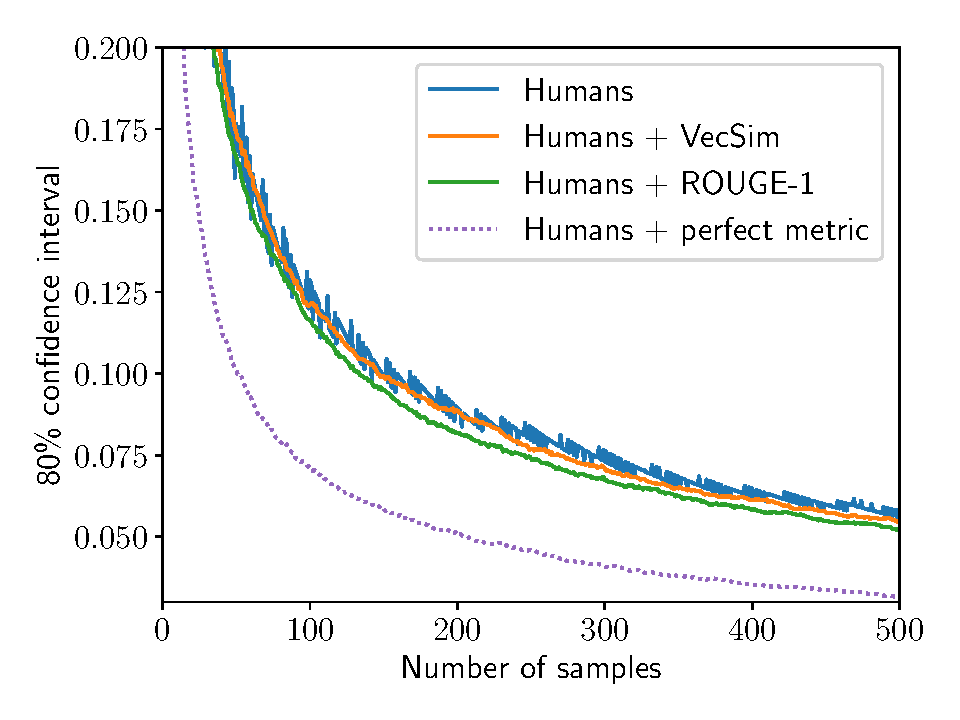
\includegraphics[width=\textwidth]{figures/msmarco_trajectory}
  \caption{\label{fig:trajectory-c}\texttt{fastqa\_ext} on MS MARCO using \texttt{AnyCorrect}}
  \end{subfigure}
  \caption{\label{fig:trajectory} 80\% bootstrap confidence interval length as a function of the number of human judgments used when evaluating the indicated systems on their respective datasets and prompts.
  (a) We see a modest reduction in variance (and hence cost) relative to human evaluation by using the VecSim automatic metric with the proposed control variates estimator to estimate \texttt{Overall} scores on the CNN/Daily Mail task; the data efficiency (DE) is $1.06$.
  (b) By improving the evaluation prompt to use \texttt{Edit}s instead, it is possible to further reduce variance relative to humans (DE is $1.15$).
  (c) Another way to reduce variance relative to humans is to improve the automatic metric evaluation; here using ROUGE-1 instead of VecSim improves the DE from $1.03$ to $1.16$.
  }
\end{figure*}

\paragraph{Results.}\footnote{%
  Extended results for other systems, metrics and prompts can be found at \url{https://bit.ly/price-of-debiasing/}.}
  
In \refsec{method} we proved that the control variates estimator is not only unbiased but also has the least variance among other unbiased estimators.
\reffig{trajectory} plots the width of the 80\% confidence interval, estimated using bootstrap, measured as a function of the number of samples collected for different tasks and prompts.
As expected, the control variates estimator reduces the width of the confidence interval. 
We measure data efficiency by the averaging of the ratio of squared confidence intervals between the human baseline and control variates estimates.
We observe that the data efficiency depends on the task, prompt and system, ranging from about 1.08 (a 7\% cost reduction) to 1.15 (a 13\% cost reduction) using current automatic metrics.

As we showed in \refsec{method}, further gains are fundamentally limited by the quality of the evaluation prompts and automatic metrics.
Figures~\ref{fig:trajectory-a} and~\ref{fig:trajectory-b} show how improving the quality of the evaluation prompt from a Likert-scale prompt for quality (\texttt{Overall}) to using post-editing (\texttt{Edit}) noticeably decreases variance and hence allows better automatic metrics to increase data efficiency.
Likewise, \reffig{trajectory-c} shows how using a better automatic metric (ROUGE-L instead of VecSim) also reduces variance.

%Note that even we were used ``a perfect metric'', i.e.\ one that had a correlation $\rho = 1$, we must collect at least a few human annotations to find out if the metric is indeed correct. \stm{I covered this case in the method section. Cut?}
%As a result, we might expect that annotator noise will still limit the data efficiency when using a perfect metric.
\reffig{trajectory} also shows the conjectured confidence intervals if we were able to eliminate noise in human judgments (noiseless humans) or have a automatic metric that correlated perfectly with average human judgment (perfect metric).
In particular, we use the mean of all (2--3) humans on each $z$ for the perfect $g(z)$ and use the mean of all humans on each $z$ for the ``noiseless'' $Y(z)$.
% AC: We want to say that the conjectured confidence intervals are an over-estimate.
%  We note that using the mean of the human responses for the perfect $g(z)$ introduces some correlation with human responses
%These probably yield optimistic \pl{maybe just remove this sentence, because we're already being optimistic; this is additional optimism, which might be confusing} data efficiencies because we don't have access to the true mean $f(z)$; further, the estimated perfect $g(z)$ we use is correlated with human judgments and hence ``corrects'' for their variance.

In both cases, we are able to significantly increase data efficiency (i.e.\ decrease estimator variance).
%but the data efficiency is capped based on the automatic metrics' correlation or the annotator noise respectively.
With zero annotator variance and using existing automatic metrics,
the data efficiency ranges from 1.42 to 1.69. With automatic metrics with perfect correlation and current variance of human judgments,
it ranges from 2.38 to 7.25.
%as shown in \reffig{data-efficiency}.
Thus, we conclude that it is important not only to improve our automatic metrics but also the evaluation prompts we use during human evaluation. 

    %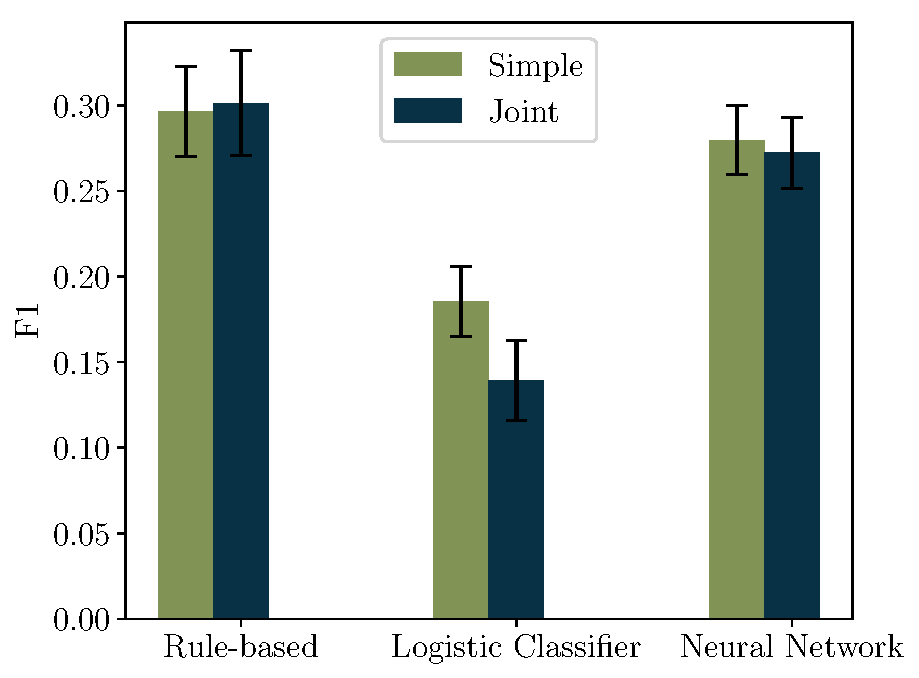
\includegraphics[width=\columnwidth]{figures/kbp2016/kbp2016_f1}
    \vfill
    \caption{\label{fig:evaluation-results}}
  \end{subfigure}

  \caption[An evaluation of the importance-reweighted estimator]{\label{fig:evaluation}
  \textbf{(a):} 
  A comparison of the number of samples used to estimate scores under the fixed and adaptive sample selection scheme.
  %In the simulation, the top 40 systems were evaluated in randomized order to achieve a target variance equal to that obtained with 500 samples for a single system.
  Each faint line shows the number of samples used during a single trial, while solid lines show the mean over 100 trials.
  The dashed line shows a square-root relationship between the number of systems evaluated and the number of samples required.
  %\ac{Note: fitting with a cubic gives $x = 0.01 y^3 -0.1y^2 + 1.8 y - 1.1$ with $R=1.0$.}
  Thus joint estimation combined with adaptive sample selection can reduce the number of labeled annotations required by an order of magnitude.
  \textbf{(b):} 
Precision ($P$), recall ($R$) and \fone{} scores from a pilot run of our evaluation service for ensembles of a rule-based system (R), a logistic classifier (L) and a neural network classifier (N) run on the TAC KBP 2016 document corpus. 
  }
\end{figure}

\section{Evaluation}
\label{sec:evaluation}

\pl{this title is totally ambiguous since this whole thesis is about evaluation;
in general, be mindful of clashes in word senses
}

Let us now see how well on-demand evaluation works in practice.
We begin by empirically studying the bias and variance of the joint estimator proposed in \refsec{method} and find it is able to correct for pooling bias while significantly reducing variance in comparison with the simple estimator.
We then demonstrate that on-demand evaluation can serve as a practical replacement for the TAC KBP evaluations by piloting a new evaluation service we have developed to evaluate three distinct systems on TAC KBP 2016 document corpus.
%We find that we are able to obtain results of  quality in a cost effective manner.

\subsection{Bias and variance of the on-demand evaluation.}
Once again, we use the labeled system predictions from the TAC KBP 2015 evaluation and treat them as an exhaustively annotated dataset.
To evaluate the pooling methodology we construct an evaluation dataset using
instances found by human annotators and labeled instances pooled from 9
randomly chosen teams (i.e.\ half the total number of participating teams), and
use this dataset to evaluate the remaining 9 teams.
On average, the pooled evaluation dataset contains between 5,000 and 6,000 labeled instances and evaluates 34 different systems (since each team may have submitted multiple systems).
Next, we evaluated sets of 9 randomly chosen teams with our proposed simple and joint estimators using a total of 5,000 samples:
about 150 of these samples are drawn from $\sY$, i.e.\ the full TAC KBP 2015 evaluation data, and 150 samples from each of the systems being evaluated.

We repeat the above simulated experiment 500 times and compare the estimated precision and recall with their true values (\reffig{simulation}).
The simulations once again highlights that the pooled methodology is biased, while the simple and joint estimators are not.
Furthermore, the joint estimators significantly reduce variance relative to the simple estimators:
the median 90\% confidence intervals reduce from 0.14 to 0.06 precision and from 0.14 to 0.08 for recall.

\subsection{Number of samples required by on-demand evaluation}
Separately, we evaluate the efficacy of the adaptive sample selection method described in \refsec{joint} through another simulated experiment.
In each trial of this experiment, we evaluate the top 40 systems in random order.
As each subsequent system is evaluated, the number of samples to pick from the system is chosen to meet a target variance and added to the current pool of labeled instances.
To make the experiment more interpretable, we choose the target variance to correspond with the estimated variance of having 500 samples.
\reffig{evaluation} plots the results of the experiment.
The number of samples required to estimate systems quickly drops off from the benchmark of 500 samples as the pool of labeled instances covers more systems.
This experiment shows that on-demand evaluation using joint estimation can scale up to an order of magnitude more submissions  than a simple estimator for the same cost.

\subsection{A mock evaluation for TAC KBP 2016}
We have implemented the on-demand evaluation framework described here as an evaluation service to which researchers can submit their own system predictions.
As a pilot of the service, we evaluated three relation extraction systems that also participated in the official 2016 TAC KBP competition.
Each system uses Stanford CoreNLP~\citep{manning2014stanford} to identify entities, the Illinois Wikifier~\citep{ratinov2011local} to perform entity linking and a combination of a rule-based system (P), a logistic classifier (L), and a neural network classifier (N) for relation extraction.
%distinct relation extraction systems (a rule-based system, a logistic classifier, and a neural network classifier) on 15,000 Newswire documents from 2016 TAC KBP evaluation.
We used 15,000 Newswire documents from the 2016 TAC KBP evaluation as our document corpus.
In total, 100 documents were exhaustively annotated for about \$2,000 and 500 instances from each system were labeled for about \$150 each.
Evaluating all three system only took about 2 hours. 

%In total, 100 documents were exhaustively annotated for about \$2,000, and 1,000 instances from each system were labeled for about \$300 each, with 500 sampled to estimate macro-averaged relation scores and 500 sampled to estimate macro-averaged entity scores.
\reffig{evaluation-results} reports scores obtained through on-demand evaluation of these systems as well as their corresponding official TAC evaluation scores.
While the relative ordering of systems between the two evaluations is the same, we note that precision and recall as measured through on-demand evaluation are respectively higher and lower than the official scores.
This is to be expected because on-demand evaluation measures precision using each systems output as opposed to an externally defined set of evaluation entities.
Likewise, recall is measured using exhaustive annotations of relations within the corpus instead of annotations from pooled output in the official evaluation.  

%We note that the rule-based system does better on \fone{} because it has significantly higher precision that the other systems, while the RNN system has the highest recall among the three systems.
%We also include TAC KBP evaluation scores for the official submissions that most closely represent these systems.
%The TAC KBP submissions are actually a combination of systems and include filtering and post-processing as required under the evaluation guidelines, e.g.\ submitting a unique instance for each relation.
%While it is hard to directly compare the two evaluation scores, we note that the our evaluation evaluates the rule-based system significantly higher: 
%, which includes submitting a unique instance for each relation, 

%\ac{@PL: Should we talk about who pays what on the platform, etc.? A reviewer mentioned this, but I don't think it's appropriate for the paper.}
% PL: yeah, leave it out
